\subsubsection{概要}
むぎまるチームは1章で述べた目標のために, 
当研究室で開発・メンテナンスをしている自己位置推定の
パッケージであるemcl2\_ros2\cite{emcl2_ros2}を使用した. 
%@@@↑これだと目標のために
%@@@(人の作った)emcl2_ros2を使ってるという感じになってよくないです. 
%@@@emcl2_ros2は自分たちでメンテナンスしてるんですから, 自分たちのものだと明記を. 
%膨張リセット\cite{ueda2004iros}による破綻の修復と
%2D LiDARのスキャンデータを用いる
%Monte Carlo localization(MCL)\cite{fox1999etal}が
%ROS 2で実装されたemcl2\_ros2\cite{emcl2_ros2}を使用した. 
emcl2\_ros2は, 膨張リセット\cite{ueda2004iros}ができる
MCL(Monte Carlo localization\cite{fox1999etal})ベースの
ROS 2パッケージである. 
膨張リセットとは, 
%自己位置が不確かなとき, 
自己位置推定になんらかの異常が検知された場合, 
これまでの推定結果をぼかすために
パーティクルの分布を膨張させる手法である. 
これにより, これまでの推定結果に問題があってパーティクルが
ロボットの位置から乖離していた場合に, 
パーティクルがロボットに近づいて, 
乖離を修正できる可能性が高くなる. 

%正確な自己位置推定へ回復する手法である. 
%広範囲に配置されたパーティクルからロボットの位置を推定するため, 破綻した自己位置の回復に効果的である. 

emcl2\_ros2は2D LiDARからの入力を想定しているため, 
3D LiDARを使う場合はデータの変換が必要となる. 
そこで, 3D LiDARのスキャンデータを高さ方向に圧縮し, 
2次元のデータとして入力とした. 
%スキャンデータの取得に2D LiDARではなく3D LiDARを用いた意図は, 
%2D LiDARでは検出不可能な高さの障害物も検出可能にするためである. 
次項で詳細に説明する. 
ちなみに, 
今後3次元のスキャンデータをemcl2\_ros2で扱えるように
拡張する予定はあるが, 今年は間に合わなかった. 

\subsubsection{システム構成}
%むぎまるチームのシステム構成について説明する. 
ロボットに搭載した計算機, センサ, アクチュエータの接続の関係及び
計算機で実行するROS 2ノードの概要を表したものを
図\ref{fig:mugimaru_system}に示す. 

Raspberry Piには, 車体制御のために, IMUとエンコーダ, 車輪駆動用のモータを接続した. 
実行するノードとしては, IMU用のROS 2ドライバノード(rt\_usb\_9axisimu\_driver)と, 
オドメトリの出力とモータの制御を実施するノード(raspimouse)がある. 
後者のノードでは, エンコーダの値と
前者のノードで配信されたIMUの情報からロボットのオドメトリを計算し, 
トピックとして配信する. 
モータの制御は, 外部のノードからトピックとして受信した
ロボットの速度指令をもとに実行する. 

ノートPCはRaspberry Piから
オドメトリのトピックを受け入れる. 
また, 3D LiDARが物理的に接続される. 
実行されるノードとしては, 3D LiDARに関係するもの: 
\begin{itemize}
	\item livox\_lidar\_publisher: Livox用のROS 2ドライバノード
	\item pointcloud\_to\_laserscan: 3D LiDARのスキャンデータを2次元に圧縮してトピックとして配信するノード
\end{itemize}
と, 自己位置推定とナビゲーションに関係するもの: 
\begin{itemize}
	\item emcl2\_ros2: 自己位置推定ノード(図中では「emcl2」と表記)
	\item navigation2\cite{nav2}のノード群: ROS 2で標準的な移動ロボットのナビゲーションパッケージに属するノード(図中では複数のノードをまとめて「navigation2」と表記)
\end{itemize}
がある. 
%%%説明がノードの話が中心になっている気がします. 
%%%~という機能を実装した. (補足として)~というノードで実装されている 的な形に直したほうがわかりやすい気がします. 
%%%
%自己位置推定には, 前項のとおりemcl2\_ros2を使用した. 
emcl2\_ros2はパラメータ以外をデフォルトの状態で使用した. 
またこのノードには, 走行する環境の地図が必要となり, 
その作成にはROS 2標準のSLAMパッケージである
slam\_toolbox\cite{slam_toolbox}を使用した. 
navigation2のグローバルプランナーとローカルプランナーではそれぞれ, 
ダイクストラ\cite{dijkstra}とDWB(dynamic window approach\cite{dwa}の
評価関数を拡張したアルゴリズム)を経路計画のアルゴリズムとして使用した. 
これらはnavigation2でデフォルトで設定されているものである. 
%@@@できれば大域計画と局所計画にどのアルゴリズム(or ノード)をつかったかも表記を

\begin{figure}[h]
  \begin{center}
    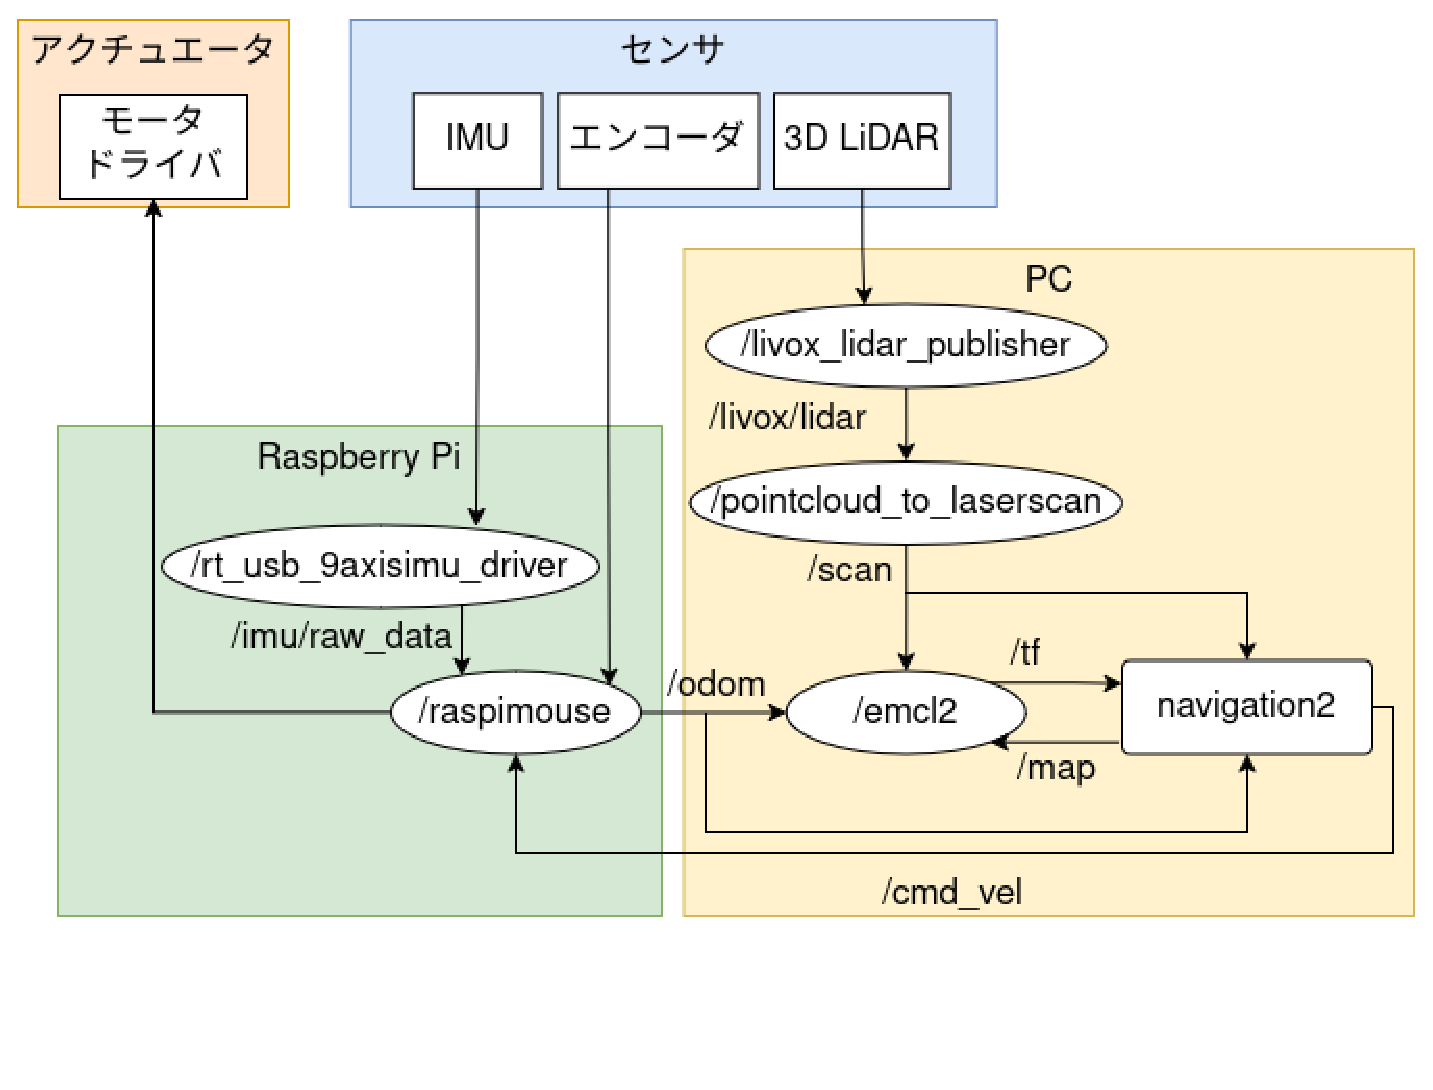
\includegraphics[width=1.0\linewidth]{figs/mugimaru_system_2024.eps}
    \caption{むぎまるチームのシステム構成}
    \label{fig:mugimaru_system}
  \end{center}
\end{figure}
%@@@↑字がちっちゃいので大きく. レイアウト変更も考えて

